%#######################################################################

In this Chapter, we present the theory of distance correlation and
justify its advantages over traditional statistics such as Pearson's
for brain parcellation. Distance correlation belongs to a family of
nonparametric statistics called energy statistics, which was first
developed by G\'{a}bor Sz\'{e}kely as a measure of dissimilarity between
probability distributions that formed the basis for nonparametric
goodness-of-fit tests. Subsequent results extended energy statistics
to problems of multivariate statistical dependence in
\cite{szekely2007measuring} and \cite{bakirov2006multivariate}.
Following this many applications of distance correlation and distance
covariance have been developed. A review of these can be found in
\cite{szekely2013energy}. Our exposition on energy statistics draws
primarily from this review.

Distance correlation is a non-linear measurement of statistical
dependency between two random variables of arbitrary dimension, and it
equals zero if and only if the two random variables are independent.
In our parcellation approach, we will compute the sample distance
correlation between each voxel and its 6 cubically adjacent neighbors
and set them as the weights of the corresponding edges. Then, edges
whose endpoints are in the same parcel can be used as a measure of the
statistical dependency between adjacent voxels in a parcel, and edges
whose endpoints lie in different parcels can be used to measure the
statistical dependency at parcel boundaries. Both our criteria for
measuring the goodness of a parcellation and the objective functions
that our algorithms seek to maximize depend on distance correlation
weights of the brain graph.

\section{Non-linear Dependencies in fMRI Data}

\begin{figure}
\caption{Pearson's and Distance Correlation for Linear and %
Non-linear Relationships}
\label{nonlinear_depend}
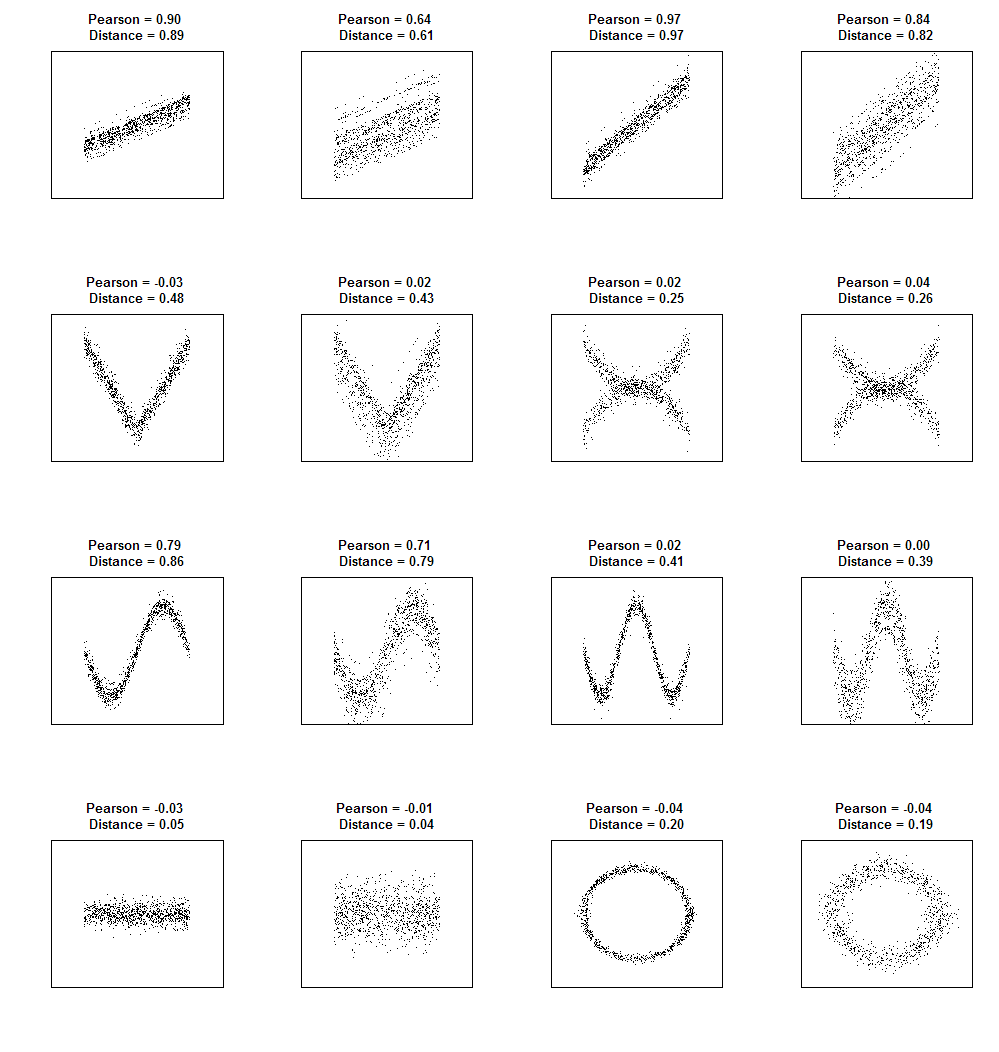
\includegraphics[scale = 0.8]{figs/1_nonlinear_depend.png}
\end{figure}

To measure dependence, statisticians have traditionally used Pearson's
correlation coefficient, in addition to the rank-based Kendall tau and
Spearman rho. These statistics work well when the underlying
relationship between the two random variables is already linear, in the
case of Pearson, or can be linear after a monotonic transformation, in
the case of Kendall and Spearman. Due to their restrictions, these
correlation coefficients will fail to capture many kinds of dependency
relationships. Figure \ref{nonlinear_depend} illustrates cases of
linear and non-linear relationships between random variables and their
sample Pearson and distance correlation values.

\begin{figure}
\caption{Four Instances of Strongly Non-Linear Relationships Between %
Adjacent Voxels in fMRI Data}
\label{fmri_nonlinear}
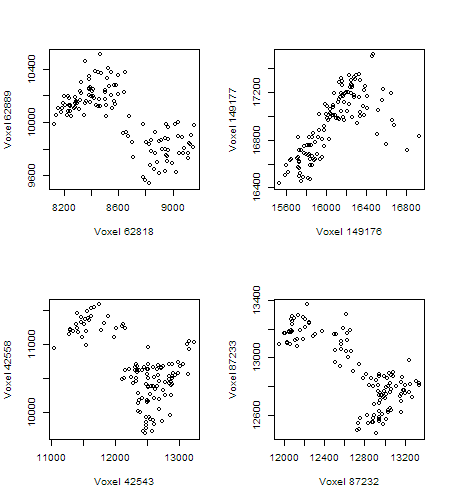
\includegraphics[scale = 0.7]{figs/1_nonlinear_ABIDE_50002.png}
\end{figure}

Non-linear dependency relationships also exist in the fMRI data. The
scatterplots in Figure \ref{fmri_nonlinear} show time samples of
spatially adjacent voxels with particularly strong non-linear
relationships.\footnote{These instances were found by searching for the
maximum difference in rank of energy distance correlation and the
coefficient of determination, or Pearson squared.} Hence using distance
correlation as the edge weights in the voxel graph has an obvious
advantage to using Pearson's correlation.

\section{Distance Covariance, Variance, and Correlation}

We first discuss the definition and properties of distance covariance,
from which the definition of distance correlation will naturally
follow. We first start with the population quantity where
$\mathcal{V}(X,Y)$ represents the population distance covariance
between two distributions, one over the random variable $X$ in a
$p$-dimensional space and the other over $Y$ in a $q$-dimensional
space.

Let $\varphi_X(s) = \Expect[e^{i s^T X}]$ denote the characteristic
function of a random vector $X$. For some positive weight function
$w : \R^p \times \R^q \mapsto [0, \infty)$ define the norm
$\|\cdot\|_w : \{\gamma : \R^p \times \R^q \mapsto \mathbb{C}\}
               \mapsto [0, \infty)$ as
\[ \|\gamma\|_w^2 = \int_{\R^{p+q}} |\gamma(s,t)|^2 w(s,t)
                    \diff s \diff t. \]

In the case where the subscript $w$ is omitted, it is implied that
$w(s,t) = 1$, the constant function taking value one. Hence
$\|\cdot\|^2$ is the typical definition of the $\ell_2$ (Euclidean)
norm squared.

\begin{definition}[Distance covariance] 
Let $X$ and $Y$ be two $p$ and $q$-dimensional (respectively) random
vectors with finite first moments and characteristic functions
$\varphi_X$ and $\varphi_Y$. Let the weight function
$w(s,t) = \dfrac{c_p c_q}{\|s\|^{1+p} \|t\|^{1+q}}$ where
$c_d = \dfrac{\Gamma(\frac{d+1}{2})}{\pi^{(d+1) / 2}}$
The \textit{squared} distance covariance between $X$ and $Y$ is defined
\begin{align*}
\mathcal{V}^2 (X,Y)
&= \| \varphi_{X,Y}(s,t) - \varphi_X(s)\varphi_Y(t) \|_w^2 \\
&= c_p c_q \int_{\R^{p+q}}
   \dfrac{|\varphi_{X,Y}(s,t) - \varphi_X(s)\varphi_Y(t)|^2}
         {\|s\|^{1+p} \|t\|^{1+q}} \diff s \diff t.
\end{align*}
Distance covariance is defined
$\mathcal{V}(X,Y) = \sqrt{\mathcal{V}^2(X,Y)}$.
\end{definition}

Distance covariance has the immediate property that
$\mathcal{V}(X,Y) = 0$ if and only if
$\varphi_{X,Y}(s,t) - \varphi_X(s) \varphi_Y(t) = 0$ for all
$s \in \R^p$ and $t \in \R^q$.

Random vectors $X$ and $Y$ are defined to be statistically independent
if and only if their joint density function $p_{X,Y}$ factors into the
product of the marginal densities of $X$ and $Y$. The one-to-one
correspondence between probability densities and characteristic
functions gives us the following:

\begin{theorem}[Kac's Theorem]
Let $X$ be $p$-dimensional and $Y$ $q$-dimensional random variables.
Then $X$ and $Y$ are independent if and only if for all $s \in \R^p$
and all $t \in \R^q$,
\[ \Expect[e^{i (s^T X + t^T Y)}]
 = \Expect[e^{i s^T X}] \Expect[e^{i t^T Y}] \]
\end{theorem}
\begin{proof}
($\implies$): If $X$ and $Y$ are independent, then
$\Expect[f(X) g(Y)] = \Expect[f(X)] \Expect[g(X)]$ for any functions
$f$ and $g$.

($\impliedby$): Let $\tilde{X}$ and $\tilde{Y}$ be independent
variables with the same marginal distribution as $X$ and $Y$. Then
\begin{align*}
\Expect[e^{i (s^T X + t^T Y)}]
&= \Expect[e^{i s^T X}] \Expect[e^{i t^T Y}] \\
&= \Expect[e^{i s^T \tilde{X}}] \Expect[e^{i t^T \tilde{Y}}] \\
&= \Expect[e^{i (s^T \tilde{X} + t^T \tilde{Y})}]
\end{align*}
The first equality comes from the premise, the second by the equal
distributions of $X$ and $\tilde{X}$, and the third by the independence
of $\tilde{X}$ and $\tilde{Y}$. Since the characteristic function
uniquely describes a distribution, $(X, Y)$ has the same joint
density function as $(\tilde{X}, \tilde{Y})$. Hence the joint density
of $X$ and $Y$ factorizes into the marginal densities.
\end{proof}

The important corrollary to this theorem is that $\mathcal{V}(X,Y) = 0$
if and only if $X$ and $Y$ are independent. Next, we define the
distance variance $\mathcal{V}(X)$

\begin{definition}
[Distance variance]
$$ \mathcal{V} (X) = \mathcal{V} (X,X) $$
\end{definition}

Analogously to the regular definitions of variance, covariance, and
correlation, the distance correlation $\mathcal{R}(X,Y)$ is

\begin{definition}
[Distance correlation]
\[ \mathcal{R} (X,Y) = \begin{cases}
  \frac{\mathcal{V}(X,Y)}{\sqrt{\mathcal{V}(X) \mathcal{V}(Y)}}
  & \text{if } \mathcal{V}(X) \mathcal{V}(Y) > 0 \\
  0 & \text{otherwise}
\end{cases} \]
\end{definition}

Distance covariance, variance, and correlation are estimated from an
independent identically distributed random sample
$\{(X_i, Y_i)\}_{i=1}^n$ by replacing the population characteristic
function with the empirical characteristic function:
\[ \widehat{\varphi}_X (t) = \frac{1}{n} \sum_{i=1}^n \exp(i t^T X_i) \]
Let $\mathcal{V}_n(X,Y)$ denote the sample distance covariance obtained
by this substitution. From \cite{szekely2007measuring} we get the
following closed-form formula for $\mathcal{V}_n(X,Y)$:

\begin{theorem}[\cite{szekely2007measuring} (Theorem 1)]
Let $\{(X_i, Y_i)\}_{i=1}^n$ be a random sample drawn iid. Define
the Euclidean distance matrices $a_{ij} = \|X_i - X_j\|$ and
$b_{ij} = \|Y_i - Y_j\|$ for $i,j$ from 1 to $n$. Define the centered
distance matrix entries
\[ A_{ij} = a_{ij} - \overline{a}_i - \overline{a}_j + \overline{a} \]
where $\overline{a}_i$ is the mean of the $i$th row (or column) of
matrix $a$ and $\overline{a}$ is the mean of all entries of $a$. Define
the centered matrix $B$ from $b$ analogously for all $i,j = 1, ..., n$.
Then,
\[ \mathcal{V}_n(X,Y) = \sqrt{\frac{1}{n^2}
                              \sum_{i,j=1}^n A_{ij} B_{ij}} \]
\end{theorem}

The sample distance variance and correlation are defined in terms of
sample distance covariance in exactly the same manner as the population
versions.

We now review some key properties that relate the sample distance
covariance to the population distance covariance that helps give
insight. We simply state the theorems and refer to the papers for
interested readers.

First, we relate the distance correlation to Pearson correlation.

\begin{definition} [$\alpha$-distance covariance] 
For $0 < \alpha < 2$
$$ \mathcal{V}_\alpha^2 (X,Y)
 = \frac{1}{C(p,\alpha) C(q,\alpha)}
   \int_{\R^{p+q}} \frac{|\varphi_{X,Y}(s,t) -
                          \varphi_X(s) \varphi_Y(t)|^2}
                        {\|s\|^{\alpha + p} \|t\|^{\alpha + q}} ds dt $$
\end{definition}

\begin{prop}[\cite{szekely2013energy} (Section 7.2)]
If $\Expect[\|X\|^\alpha] + \Expect[\|Y\|^\alpha] < \infty$ then
$$ \mathcal{V}_\alpha^2 (X,Y) = \Expect[ \|X - X'\|^\alpha \|Y - Y'\|^\alpha ] + \Expect \|X - X'\|^\alpha \Expect \|Y - Y'\|^\alpha - 2 \Expect[ \|X - X'\|^\alpha \|Y - Y''\|^\alpha ]$$

In particular, if $\alpha = 2$, $p = q = 1$, the distance correlation is 
the absolute value of Pearson's correlation coefficient.
\end{prop}

Next, we show statement ensuring consistency under the existence of the
first moments.

\begin{prop}[\cite{szekely2007measuring} (Corollary 1)]
If $\mathbb{E}(\|X\| +\|Y\|)< \infty$, then almost surely
\[
\lim_{n\rightarrow\infty}\widehat{\mathcal{R}}(X,Y) = \mathcal{R}(X,Y)
\]
\end{prop}

While we did not find a theorem explicitly stating the rate of 
convergence, the above theorem gives us satisfaction that if
$\mathcal{V}(X,Y)=0$ (meaning $X$ and $Y$ are independent), then as long 
as we have enough samples, $\widehat{\mathcal{V}}(X,Y) $ will approach
0. In our case, $n$ refers to the number of time samples which
typically range from $n=100$ to $n=200$.

We next show the asymptotic distribution of the sample distance
covariance under independence of $X$ and $Y$. While this is not used in
our work (as we do not apply the hypothesis test), this can inspire
future work where instead of computing the sample energy statistics
$\widehat{\mathcal{V}}(X,Y)$, we compute the $p$-value
under the null hypothesis $H_0: X \indep Y$.

To formulate the asymptotic distribution, we need additional notation.
Let $Q$ be a random variable where
\[ Q \overset{D}{=} \sum_{j=1}^{\infty}\lambda_j Z^2_j, \]
where $Z_j$ are independent, standard normal random variables and
$\{\lambda_j\}$'s are nonnegative constants dependent on the
characteristic functions on the joint distribution $(X,Y)$ such that
$\mathbb{E}[Q] = 1$. Here, we put the superscript $D$ to denote equality 
in distribution.

\begin{prop}[\cite{szekely2007measuring} (Corollary 2)]
If $\mathbb{E}(\|X\| +\|Y\|)< \infty$, then
\begin{itemize}
\item If $X$ and $Y$ are independent, then $n\widehat{\mathcal{V}}^2/S_2 \overset{D}{\rightarrow} Q$.
\item If $X$ and $Y$ are dependent, then $n\widehat{\mathcal{V}}^2/S_2 \overset{P}{\rightarrow} \infty$.
\end{itemize}
\end{prop}

Here, the superscript $D$ and $P$ denote convergence in distribution and
probability as $n$ goes to infinity. More explicit asymptotic
distributions are given in \cite{szekely2013energy} when $X$ and $Y$ are
Gaussian, but in general, bootstrapping procedures can be used to test
this hypothesis. Similar procedures can be derived on the distance
correlation.

In all our computations throughout our thesis, we use the \texttt{dcor}
function in the \texttt{energy} package to compute the distance
correlation efficiently.
